\documentclass{acmsiggraph}                     % final
%\documentclass[annualconference]{acmsiggraph}  % final (annual conference)
%\documentclass[review]{acmsiggraph}            % review
%\documentclass[widereview]{acmsiggraph}        % wide-spaced review
%\documentclass[preprint]{acmsiggraph}          % preprint

%% Uncomment one of the five lines above depending on where your paper is
%% in the conference process. ``review'' and ``widereview'' are for review
%% submission, ``preprint'' is for pre-publication, and ``final'' is for
%% the version to be printed. The ``final'' variant will accept the 
%% ``annualconference'' parameter, which changes the height of the space
%% left clear for the ACM copyright information.

%% The 'helvet' and 'times' packages define the typefaces used for
%% serif and sans serif type in this document. Computer Modern Roman 
%% is used for mathematics typesetting. The scale factor is set to .92
%% to bring the sans-serif type in line with the serif type.

\usepackage[scaled=.92]{helvet}
\usepackage{times}

%% The 'graphicx' package allows for the inclusion of EPS figures.

\usepackage{graphicx}

%% use this for zero \parindent and non-zero \parskip, intelligently.

\usepackage{parskip}

%% Optional: the 'caption' package provides a nicer-looking replacement
%% for the standard caption environment. With 'labelfont=bf,'textfont=it',
%% caption labels are bold and caption text is italic.

\usepackage[labelfont=bf,textfont=it]{caption}

%% If you are submitting a paper to the annual conference, please replace 
%% the value ``0'' below with the numeric value of your OnlineID. 
%% If you are not submitting this paper to the annual conference, 
%% you may safely leave it at ``0'' -- it will not be included in the output.

\onlineid{0}

%% Paper title.

\title{A Study of Immersion Factors Using an Augmented Reality Simulation}

%% Author and Affiliation (single author).

%%\author{Roy G. Biv\thanks{e-mail: roy.g.biv@aol.com}\\Allied Widgets Research}

%% Author and Affiliation (multiple authors).

\author{
%Roy G. Biv\thanks{e-mail: roy.g.biv@aol.com}\\ Starbucks Research %
%\and Ed Grimley\thanks{e-mail:ed.grimley@aol.com}\\Nigel Mansell\thanks{nigelf1@msn.com}\\ Grimley Widgets, Inc. %
%\and Martha Stewart\thanks{e-mail:martha.stewart@marthastewart.com}\\ Martha Stewart Enterprises \\ Microsoft Research}
}

%% Keywords that describe your work.

\keywords{
%radiosity, global illumination, constant time
}

%%%%%% START OF THE PAPER %%%%%%

\begin{document}

%\teaser{
%  \includegraphics[width=1.5in]{sample.eps}
%  \caption{Lookit! Lookit!}
%}

%% The ``\maketitle'' command must be the first command after the
%% ``\begin{document}'' command. It prepares and prints the title block.

\maketitle

%% Abstract section.

\begin{abstract}
%It is extremely challenging to run controlled studies comparing multiple augmented reality (AR) systems.  We use an �AR simulation� approach, in which a virtual reality (VR) system is used to simulate multiple AR systems. In order to validate this approach, we carefully replicated a well-known study by Ellis et al. using our simulator, obtaining comparable results. 

In a second study using the AR simulator, we studied a tracking task where the AR interface provides x-ray vision to help track a moving target.  We varied the field of view of the AR display, as well as the reliability of the head tracker.  In low reliability conditions, we simulate tracker failure by disabling the augmented view of the scene for brief periods.  Our study gives insight into the effect of head tracker reliability on user performance in a tracking task, as well as the relationship between reliability and field of view in an AR system.

\end{abstract}

%% ACM Computing Review (CR) categories. 
%% See <http://www.acm.org/class/1998/> for details.
%% The ``\CRcat'' command takes four arguments.

\begin{CRcatlist}
%  \CRcat{K.6.1}{Management of Computing and Information Systems}{Project and People Management}{Life Cycle};
%  \CRcat{K.7.m}{The Computing Profession}{Miscellaneous}{Ethics}
\end{CRcatlist}

%% The ``\keywordlist'' command prints out the keywords.
\keywordlist

\section{Introduction}

%% The ``\copyrightspace'' command must be the first command after the 
%% start of the first section of the body of your paper. It ensures the
%% copyright space is left at the bottom of the first column on the first
%% page of your paper.

%% \copyrightspace

Augmented Reality systems may be used to simulate x-ray vision \cite{1383060}.  The ability to see through solid objects has applications in various fields ranging from engineering and architecture to military or search-and-rescue operations.  Unfortunately, implementing x-ray vision is not a trivial task.  AR systems have cost issules, including those pertaining to level-of-immersion.  For example, what is the ideal augmented field of view (FOV) for a given scenario?  Other issues relate to tracking the objects in the x-ray view, such as GPS dropout errors \cite{4079263}, where tracking is temporarily lost.

In this paper, we study the effects of varying augmented FOV along with object-tracking dropouts.  By using an AR simulation built with virtual reality, it is possible to simulate the tracking dropouts, which would otherwise be difficult or impossible to replicate.  The simulation is a tracking task, where the participant is placed inside a virtual room and visually follows a person outside, walking an unpredictable path.  We wish to answer the following questions.  What effect does varying the augmented FOV have on user tracking performance?  What effect do different dropout lengths have on performance?  What are the interactions between these two variables?

\section{Related Work}

Livingston and Ai \cite{4637329} studied the effects of various sources of registration error with an AR simulation similar to our own.  Here, participants tracked a virtual car moving throughout a real environment, with a white box representing an augmented view of the car's location.  A white box was continuously visible, even when the car itself was occluded by a building in the environment.  Other virtual cars and their associated white boxes acted as distractors.  At specific times during the experiment, the simulation would freeze and the participant was asked to align the center of their view (indicated by cross-hairs) on the location of the correct car and press a key.  While the effects of several types of error were studied in this work, the effect of registration dropouts was not examined.

Bane and Hollerer \cite{1383060} propose a set of AR tools for virtual x-ray vision.  Various augmented views are presented, each attempting to overcome the "Superman's X-ray vision" problem of presenting too much AR information to the user.  The toolset's usefulness is illustrated with an example of an outdoors user viewing the contents of a nearby building.

other studies which vary AR fov, tracking failures

previous X-ray AR work

simulated AR

\cite{4637329,4811058,1383060}

\section{AR Simulation}

Our experiment involves a tracking task which uses an augmented reality interface to allow people to be tracked behind walls.  A participant stands in the middle of a square room with doors and windows on all sides.  Outside of the room, people are walking around the building.  The target person to be tracked is visually distinguishable by a large black top hat.  The augmented reality interface overlays a translucent red rectangle on each person, which is visible even when the person is occluded by a wall.  However, the target person's overlay is not different from any other person's overlay; the target is only identifiable when visible through a window or a door.

To actually run this experiment using a true augmented reality system would be difficult.  Many confederates would be needed to walk around the room, and their movements would need to be accurately reproduced for each new participant.  Also, the confederates would need to be continously tracked for the augmented overlays to be displayed.  Instead, we simulated the experiment setup in a completely virtual environment.

By simulating augmented reality, we are freed from the current restrictions of tracking and display technology.  Using a simulated environment also makes the experiment more controllable, and thus more easily reproduced.

\section{Experimental Design}

\begin{figure}[ht!]
	\centering
	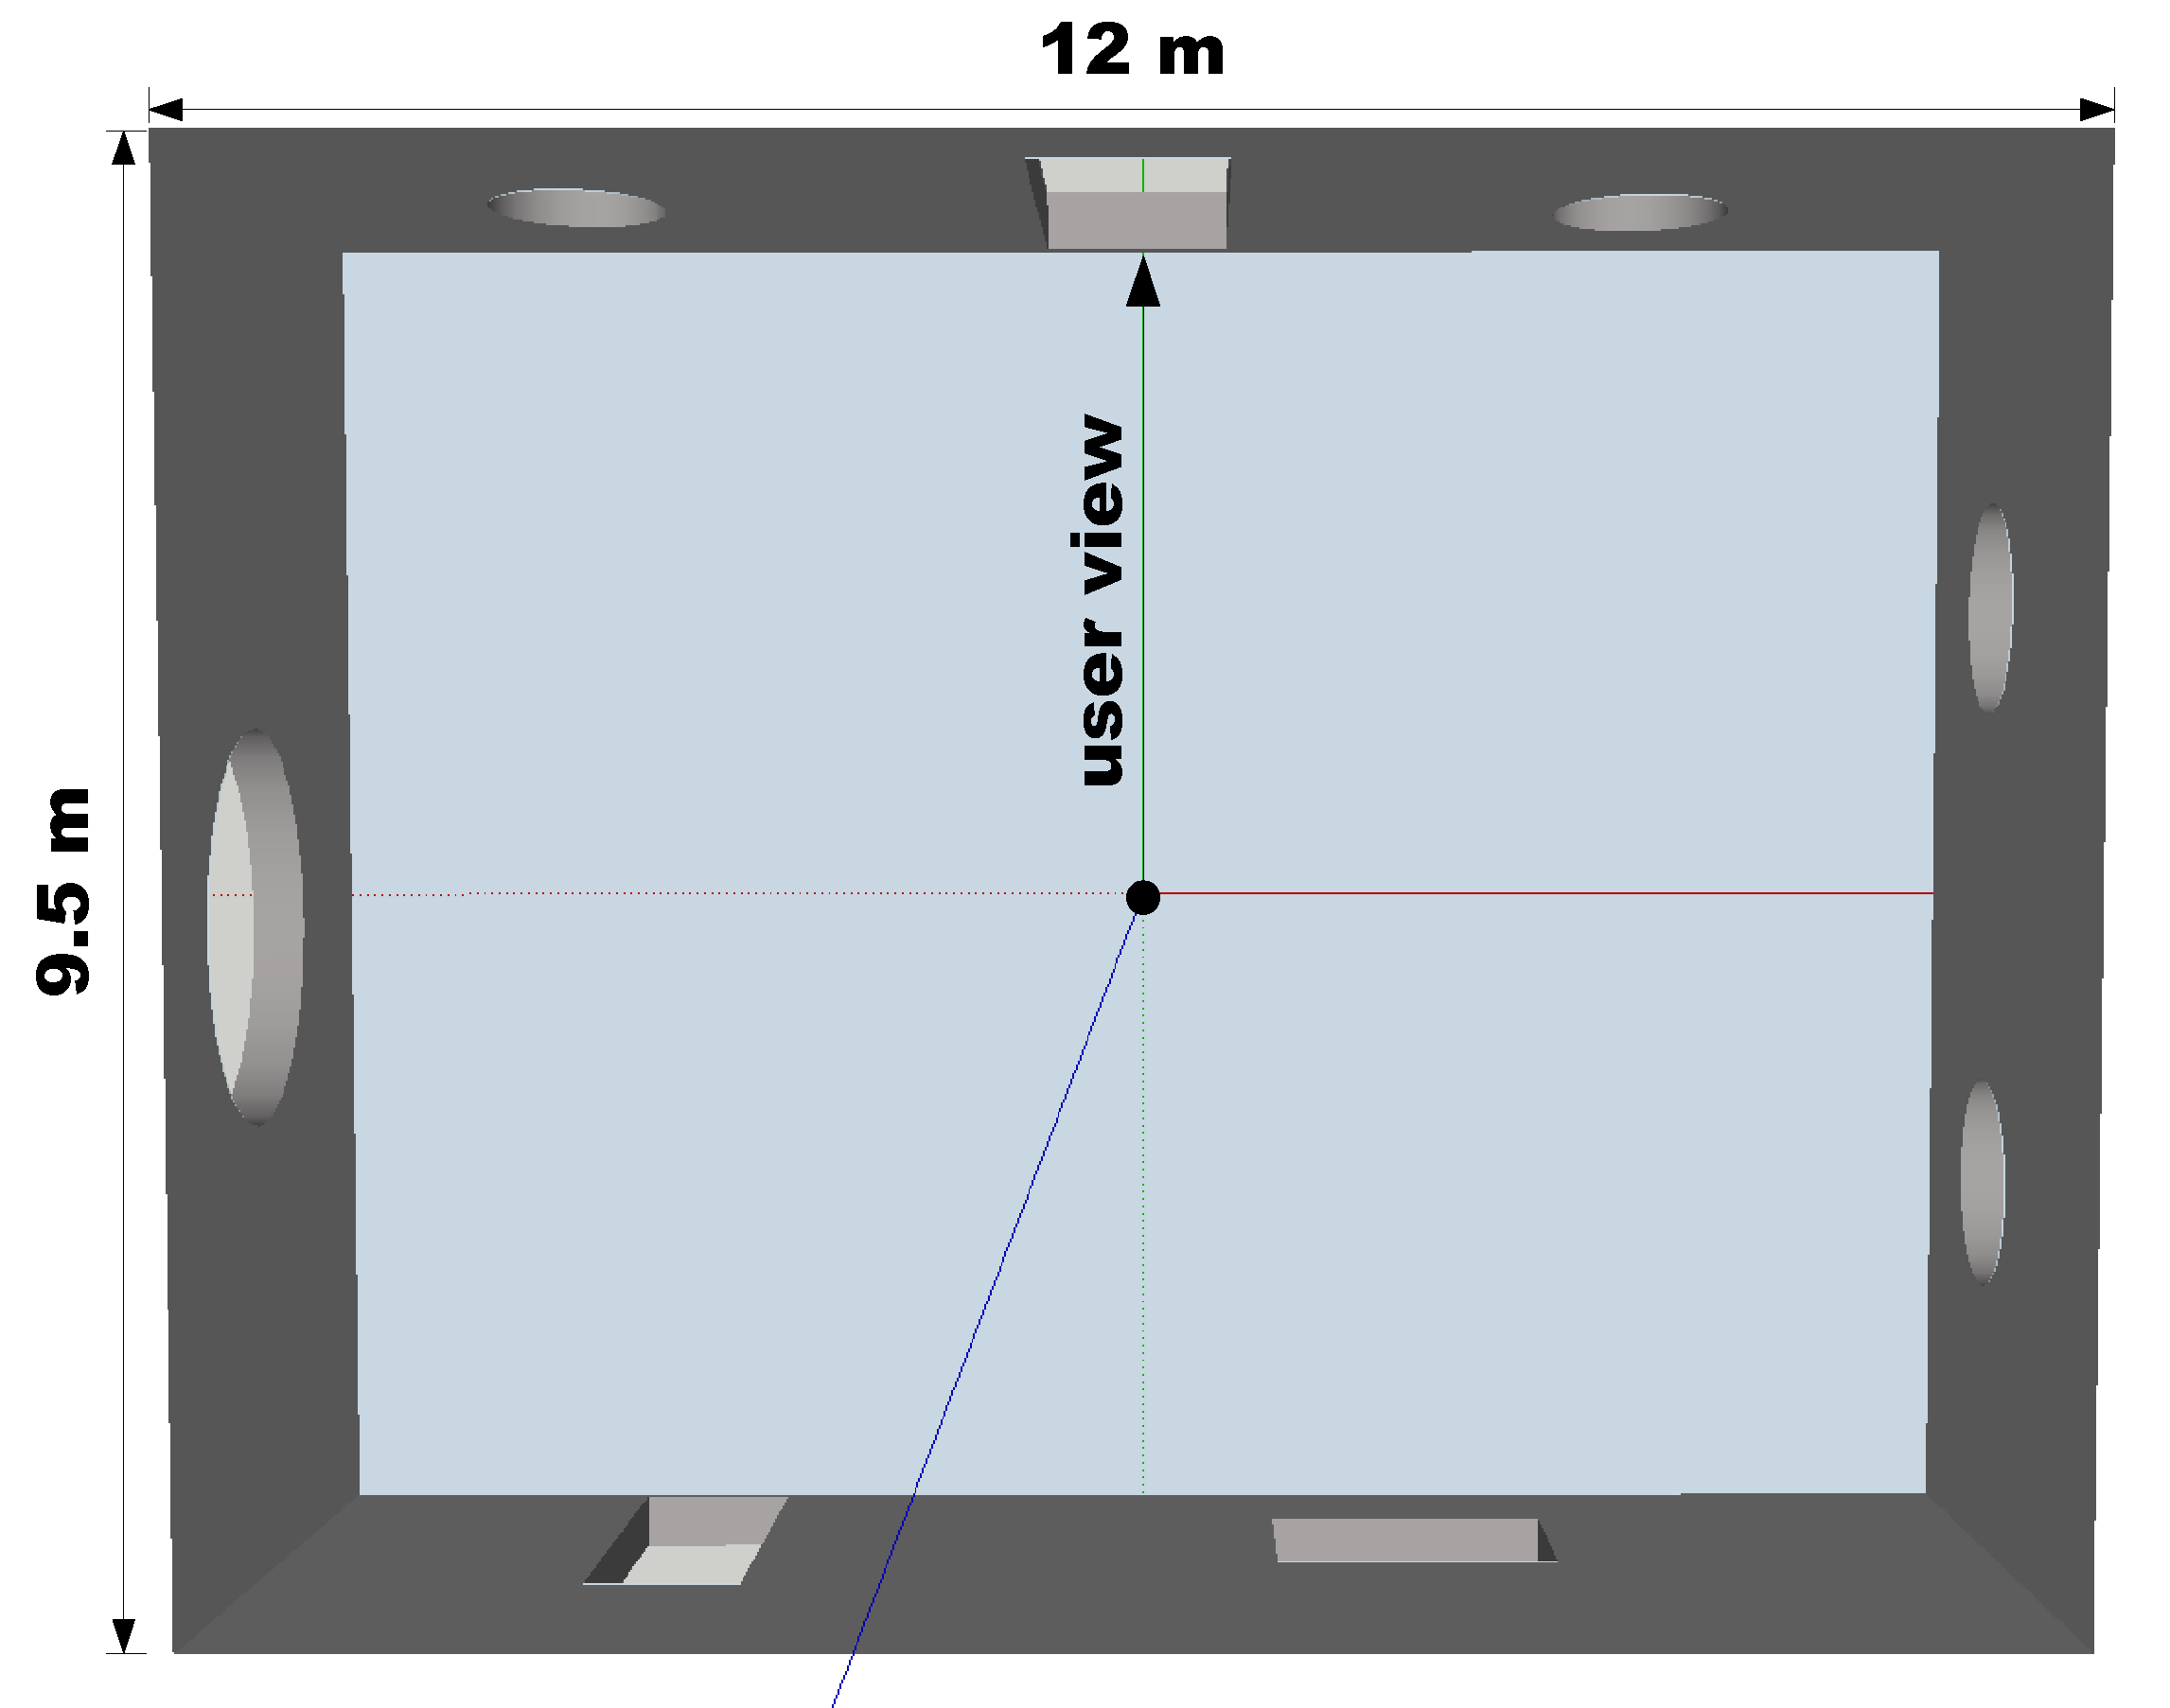
\includegraphics[width=3.5in]{figures/augmentedroom.png}
	\caption{Overhead view of virtual room (approx. measure).  Participant is stationary in the center of the room, with initial orientation along ``user view'' arrow.  Top-hat's initial position is outside the front doorway, directly in the participant's view.}
\end{figure}

Participants are presented a view of the scene through a head-mounted display helmet with orientation tracking.  The tracking overlays are  augmented on top of the image to form the simulated augmented reality view.

The parameters of our experiment are divided between the ``real'' immersion factors, such as the field of view of the HMD, and the ``augmented'' immersion factors, such as the field of view of the simulated AR display, and the performance of the head tracker.  We introduce periods of tracking failure, where the augmented overlays disappear, to simulate the effect of failures in a real tracking system.  For example, such failures might occur with a magnetic tracker near interfering materials, or with visual tracking when tracked features are lost.

In our experiment we vary two parameters: the field of view of the AR interface and the length of tracking failure periods.  Each trial lasted sixty seconds, and had seven tracking failures.  The total vertical field of view of our HMD is 36 degrees; the three possible values for the augmented field of view were 10, 20, and 34 degrees.  We varied the length of tracking failures between two seconds, one second and zero seconds (no failure).  We experimented with longer values but deemed them too long to be realistic through expert analysis.  This gave us a total of 9 conditions, and for each participant we tested each condition 3 times giving a total of 27 trials per participant.

During each trial there are 20 people in addtition to the man wearing the tophat waking around outside of the room.  The walking path for each person was given by a randomly generated set of points with the constraint that they must stay within the rectangular area of size X by X surrounding the room.  At each point in the path the person would randomly change his walking speed to a new value which was within a range we deemed accecptable through expert analysis.  The man wearing the tophat had the additional constraints as follows.  He must start at the same location for each trial which made him visible by the participant through the door shaped opening in the building.  In order to make the paths by of similar dificulty we decided, through expert analysis, that through the trial he must have walked around the entire building at least once, and he must be visible through the windows for at least $x$ seconds.  We made sure these constraints were met by randomly generating paths until they were satisfied.  We generated 27 sets of patahs this way, one for each trail.  We used a balanced latin square to order these paths and the conditions to discourage the effects of learning.

The experiment was written in Python using the Vizard environment.  Tracking was done using InterSense InertiaCube3 orientation tracker which has 180 Hz update rate.  We used a Pro-View 60 head mounted display which displays $640\times480$ video at 60 Hz, and has 36 degrees vertical field of view.  We did not use stereoscopic display.  We ran the experiment on a 2.4 GHz Intel Core 2 machine with 2 Gb of RAM and a NVIDIA GeForce 9800 GX2 graphics card running Windows XP.

\section{Analysis}

In our experiment we define performance as effectiveness in tracking the top hat character.  We measure performance by recording the angular distance (in yaw) between the the user's viewing direction and the direction towards the target character.  This measure ranges between zero and 180 degrees (we used the smaller of the two options, clockwise and counter-clockwise).  We record one measurement per video frame, at about sixty frames per second, resulting in about 3600 measurements for a one second trial.

Because the video does not run at exactly 60 Hz, each trial might have a slightly different number of measurements.  We also record a timestamp for each measurement, so that we can determine their exact frequency.  As a pre-processing step, we linearly re-sample the data for each trial so that each has exactly 3600 measurements at 60 Hz.

We observed that participants tend to switch between two different states during the experiment: a tracking state, where they are following the target; and a lost state, where they are searching for the target.  The two states are easily visible in the data.  In the tracking state, the angular error is generally low.  We asked participants to keep the cross hairs on the target as closely as they could, but different participants achieved different levels of accuracy.  In the lost state, the error starts to steadily climb, and may fluctuate depending on where the target moves.  The error may even return to near-zero during a lost state, if the participant unwittingly crosses the target's path.

We hypothesize that less immersive conditions will have longer and more frequent periods where the participant is lost.  We considered several different metrics which might be appropriate in testing this hypothesis.

The simplest is the average error over an entire trial.  However, this may not accurately capture the amount that a participant is lost, because the error does not necessarily stay high during the lost state, and also different participants may generally keep the cross hair further from the target even in the tracking state.

We can more explicitly detect the lost state by applying a threshold $\tau$ to the data.  When the error rises above the threshold, we consider the participant lost.  TODO: how to determine this threshold??

One metric which uses this threshold is the ``time to failure,'' the time until a lost state is encountered.  However a participant may reach the lost state sooner or later depending on the movement of the avatars.  We also considered a measurement we called ``time tracking,'' which is the amount of time spent in the tracking state.  This metric seems to most clearly represent how well a participant performed.  Trials with either more lost periods or longer lost periods will result in a lower total time tracking.

\begin{figure}[ht!]
	\centering
	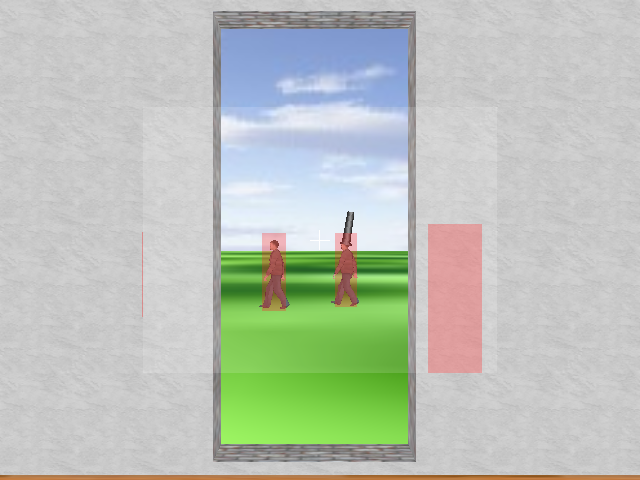
\includegraphics[width=3.5in]{figures/tophatscreenshot.png}
	\caption{Sample user-view of AR simulation.  Top-hat is visible (non-occluded) in the doorway.  The augmented view overlays transparent red rectangles on the characters, indicating their location while occluded.}
\end{figure}

\section{Results}

\section{Conclusions and Future Work}

\section*{Acknowledgements}

\bibliographystyle{acmsiggraph}
\nocite{*}
\bibliography{paper}
\end{document}
